\section{Contact Conditions Between Particles}\label{sec:contact-conditions}

In contrast to free surfaces, where the geometric evolution of a node is not constrained by the surrounding space, in grain boundaries the node shifting acts counter the solid material of the other particle.
This introduces additional constraints, since the grain boundary must not form holes and must not overlap.
The geometric constraints are dependent on the local evolution of the grain boundary nodes, as well as the relative position change of the particles.

Starting from a compact grain boundary, meaning that there are no holes and/or overlap present within it, the condition of maintaining the compactness of the grain boundary can be formulated as follows, if the postions of the particles are fixed.

\begin{subequations}
    \begin{align}
        \Step\Shift_{\Normal}\Regarding1 = \Step\Shift_{\Normal}\Regarding2 \\
        \Step\Shift_{\Tangential}\Regarding1 = \Step\Shift_{\Tangential}\Regarding2
        \label{eq:maintain-compact-particles-fixed}
    \end{align}
\end{subequations}

But in reality the positions of particles to each other change, which can be observed macroscopically as shrinkage.
So we formulate instead the total displacement of a node in absolute cartesian space, which must be equal regarded from both particles.

\begin{subequations}
    \begin{align}
        \Step\X_{\Particle1} + \Step\X_{\Normal}^{\Regarding1} + \Step\Y_{\Normal}^{\Regarding1}
        &= \Step\X_{\Particle2} + \Step\X_{\Normal}^{\Regarding2} + \Step\Y_{\Normal}^{\Regarding2}\\
        \Step\X_{\Particle1} + \Step\X_{\Tangential}^{\Regarding1} + \Step\Y_{\Tangential}^{\Regarding1}
        &= \Step\X_{\Particle2} + \Step\X_{\Tangential}^{\Regarding2} + \Step\Y_{\Tangential}^{\Regarding2}
        \label{eq:absolute-displacement-contact-constraints}
    \end{align}
\end{subequations}

\begin{figure}
    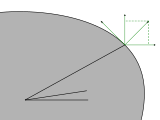
\includegraphics{img/model_development/node_shift_global}
    \caption{Geometric Conditions for Global Node Displacement}
    \label{fig:model_development/node_shift_global}
\end{figure}

As can be seen from \autoref{fig:model_development/node_shift_global}, the angles of projection of the normal and tangential node shifting to the global cartesian axes are as follows:

\begin{subequations}
    \begin{align}
        \eta_{\Normal} &= \RotationAngle + \Angle + \left( \SurfaceRadiusAngle_{\Lower} + \SurfaceVectorAngle_{\Normal\Lower} - \PI \right)
        \label{eq:global-shift-normal-angle} \\
        \eta_{\Tangential} &= \left( \PI - \SurfaceRadiusAngle_{\Lower} + \SurfaceVectorAngle_{\Tangential\Lower} \right) - \RotationAngle - \Angle
        \label{eq:global-shift-tangential-angle}
    \end{align}
\end{subequations}

With these and further identities on the trigonometric functions the displacements of the node are given as follows:

\begin{subequations}
    \begin{align}
        \Step\X_{\Normal} &= -\Step\Shift_{\Normal} \cos \left( \RotationAngle + \Angle + \SurfaceRadiusAngle + \SurfaceVectorAngle \right)
        \label{eq:global-shift-normal-x} \\
        \Step\Y_{\Normal} &= -\Step\Shift_{\Normal} \sin \left( \RotationAngle + \Angle + \SurfaceRadiusAngle + \SurfaceVectorAngle \right)
        \label{eq:global-shift-normal-y} \\
        \Step\X_{\Tangential} &= \Step\Shift_{\Tangential} \cos \left( \RotationAngle + \Angle + \SurfaceRadiusAngle + \SurfaceVectorAngle \right)
        \label{eq:global-shift-tangential-x} \\
        \Step\Y_{\Tangential} &= \Step\Shift_{\Tangential} \sin \left( \RotationAngle + \Angle + \SurfaceRadiusAngle + \SurfaceVectorAngle \right)
        \label{eq:global-shift-tangential-y}
    \end{align}
\end{subequations}

Inserted in \autoref{eq:absolute-displacement-contact-constraints} this leads to two additional constraints for each grain boundary and neck node, which define the particle displacements $\Step\X_{\Particle i}$ and $\Step\Y_{\Particle i}$ of each particle except one.
A sole particle per contact group must be fixed in space by constraining its displacements to zero.
